\documentclass{beamer}\usepackage[]{graphicx}\usepackage[]{color}
%% maxwidth is the original width if it is less than linewidth
%% otherwise use linewidth (to make sure the graphics do not exceed the margin)
\makeatletter
\def\maxwidth{ %
  \ifdim\Gin@nat@width>\linewidth
    \linewidth
  \else
    \Gin@nat@width
  \fi
}
\makeatother

\definecolor{fgcolor}{rgb}{0.345, 0.345, 0.345}
\newcommand{\hlnum}[1]{\textcolor[rgb]{0.686,0.059,0.569}{#1}}%
\newcommand{\hlstr}[1]{\textcolor[rgb]{0.192,0.494,0.8}{#1}}%
\newcommand{\hlcom}[1]{\textcolor[rgb]{0.678,0.584,0.686}{\textit{#1}}}%
\newcommand{\hlopt}[1]{\textcolor[rgb]{0,0,0}{#1}}%
\newcommand{\hlstd}[1]{\textcolor[rgb]{0.345,0.345,0.345}{#1}}%
\newcommand{\hlkwa}[1]{\textcolor[rgb]{0.161,0.373,0.58}{\textbf{#1}}}%
\newcommand{\hlkwb}[1]{\textcolor[rgb]{0.69,0.353,0.396}{#1}}%
\newcommand{\hlkwc}[1]{\textcolor[rgb]{0.333,0.667,0.333}{#1}}%
\newcommand{\hlkwd}[1]{\textcolor[rgb]{0.737,0.353,0.396}{\textbf{#1}}}%
\let\hlipl\hlkwb

\usepackage{framed}
\makeatletter
\newenvironment{kframe}{%
 \def\at@end@of@kframe{}%
 \ifinner\ifhmode%
  \def\at@end@of@kframe{\end{minipage}}%
  \begin{minipage}{\columnwidth}%
 \fi\fi%
 \def\FrameCommand##1{\hskip\@totalleftmargin \hskip-\fboxsep
 \colorbox{shadecolor}{##1}\hskip-\fboxsep
     % There is no \\@totalrightmargin, so:
     \hskip-\linewidth \hskip-\@totalleftmargin \hskip\columnwidth}%
 \MakeFramed {\advance\hsize-\width
   \@totalleftmargin\z@ \linewidth\hsize
   \@setminipage}}%
 {\par\unskip\endMakeFramed%
 \at@end@of@kframe}
\makeatother

\definecolor{shadecolor}{rgb}{.97, .97, .97}
\definecolor{messagecolor}{rgb}{0, 0, 0}
\definecolor{warningcolor}{rgb}{1, 0, 1}
\definecolor{errorcolor}{rgb}{1, 0, 0}
\newenvironment{knitrout}{}{} % an empty environment to be redefined in TeX

\usepackage{alltt}
%\documentclass[handout]{beamer}
%\usepackage[dvips]{color}
\usepackage{graphicx}
\usepackage{amsmath,amssymb,array,comment,eucal}
\usepackage{xcolor}
\definecolor{beamer@blendedblue}{RGB}{86,155,189}
\definecolor{myblue}{RGB}{12,76,138}
\setbeamercolor{structure}{fg=myblue}
\definecolor{Ftitle}{RGB}{12,76,138}
\definecolor{Descitem}{RGB}{238,238,244}
\definecolor{StdTitle}{RGB}{12,76,138}
\definecolor{StdBody}{RGB}{213,24,0}
\definecolor{StdBody}{RGB}{213,24,0}

\definecolor{AlTitle}{RGB}{255, 190, 190}
\definecolor{AlBody}{RGB}{213,24,0}

\definecolor{ExTitle}{RGB}{201, 217, 217}
\definecolor{ExBody}{RGB}{213,24,0}

\setbeamercolor{frametitle}{fg = Ftitle}
\setbeamercolor{title}{fg = Ftitle}
\setbeamercolor{item}{fg = Ftitle}
\setbeamercolor{subitem}{fg = Ftitle}
\setbeamercolor{subsubitem}{fg = Ftitle}
\setbeamercolor{description item}{fg = myblue}
\setbeamercolor{titlelike}{fg=myblue}

%$Id: macros.tex,v 1.2 2006/02/13 14:23:55 rlw Exp rlw $
\newcommand{\Lmea}{{\cal L}} 
\newcommand{\scale}{\bflambda} 
\newcommand{\Scale}{\bfLambda} 
\newcommand{\bfscale}{\bflambda} 
\newcommand{\mean}{\bfchi}
\newcommand{\loc}{\bfchi}
\newcommand{\bfmean}{\bfchi}
\renewcommand{\k}{g}
\newcommand{\Gen}{{\cal G}}
\newcommand{\eps}{\epsilon}

\newcommand{\ind}{\mathrel{\mathop{\sim}\limits^{\mathit{ind}}}}
\newcommand{\iid}{\mathrel{\mathop{\sim}\limits^{\mathit{iid}}}}
\newcommand{\dis}{\mathrel{\mathop{=}\limits^{d}}}
\newcommand{\sgn}{\mathop{\rm sgn}}
\newcommand{\cmp}{h}
\newcommand{\dbdo}{d\beta ~ d\omega}
\newcommand{\real}{{\mathbb{R}}}
\newcommand{\Ber}{\mbox{\rm Ber}}
\newcommand{\GP}{\mbox{\rm GP}}
\newcommand{\SaS}{\text{S$\alpha$S}}
\newcommand{\RA}{{\real \times A}}
\newcommand{\RK}{{\real \times K}}
\newcommand{\RO}{{\real \times \Omega}} 
\newcommand{\RS}{{\bbR \times \LamS}}
  \newcommand{\set}[1]{\left\{#1\right\}}
  \newcommand{\bet}[1]{\left[#1\right]}
  \newcommand{\cet}[1]{\left(#1\right)}
%  \renewcommand{\half}{{\scriptstyle\frac12}}
\newcommand{\subA}{(\eps_1 < \beta \le \eps_2) \times \LamS}
 \newcommand{\uu}{{\big(\scale(x - \loc)\big)}}
 \newcommand{\uuj}{{\big(\scale_j(x-\loc_j)\big)}}
 \newcommand{\bbT}{{\mathbb{T}}}
 \newcommand{\ui}{{[0,1)}}
 \newcommand{\spq}[1]{\left|#1\right|^s_{pq}}
 \newcommand{\spqper}[1]{\left|#1\right|^{s\,*}_{pq}}
 \newcommand{\sspqper}[1]{\left\|#1\right\|^{s\,*}_{pq}}
 \newcommand{\sspq}[1]{\left\|#1\right\|^s_{pq}}    % Besov semi-norm
 \newcommand{\qp}[1]  {\left\|#1\right\|^q_p}         % Hilbert-space norm
 \newcommand{\qper}[1]{\left\|#1\right\|^{*\,q}_p}  % Periodic HS norm
 

\newcommand{\bbW}{{\mathbb{W}}}
\newcommand{\bbB}{{\mathbb{B}}}
\newcommand{\Sob}{{\ensuremath{\bbW^s_2}}}
\newcommand{\Besov}{{\ensuremath{\bbB^s_{pq}}}}
\newcommand{\Besper}{{\ensuremath{\bbB^{s\,*}_{pq}}}}
\newcommand{\Sobx}[1]{{\bbW^{#1}_2}}
\newcommand{\Besovx}[1]{{\bbB^{#1}_2}}
\newcommand{\SN}[1]{\|{#1}\|_\Sob}
% MATH LETTER DEFINITIONS
\newcommand{\Levy}{L{\'e}vy}
\newcommand{\nmathbf}{\bm}
\newcommand{\tabb}[1]{\hspace*{#1\parindent}}
%\newcommand{\G}{{g}}    % Really the same as \GB
\newcommand{\g}{{\phi}} %\newcommand{\g}{{g}}
\newcommand{\GB}{{g}}  
% Roman math Bold face 


\def\bfA{\nmathbf A}
\def\bfB{\nmathbf B}
\def\bfC{\nmathbf C}
\def\bfD{\nmathbf D}
\def\bfE{\nmathbf E}
\def\bfF{\nmathbf F}
\def\bfG{\nmathbf G}
\def\bfH{\nmathbf H}
\def\bfI{\nmathbf I}
\def\bfJ{\nmathbf J}
\def\bfK{\nmathbf K}
\def\bfL{\nmathbf L}
\def\bfM{\nmathbf M}
\def\bfN{\nmathbf N}
\def\bfO{\nmathbf O}
\def\bfP{\nmathbf P}
\def\bfQ{\nmathbf Q}
\def\bfR{\nmathbf R}
\def\bfS{\nmathbf S}
\def\bfT{\nmathbf T}
\def\bfU{\nmathbf U}
\def\bfV{\nmathbf V}
\def\bfW{\nmathbf W}
\def\bfX{\nmathbf X}
\def\bfY{\nmathbf Y}
\def\bfZ{\nmathbf Z}

\def\bfa{\nmathbf a}
\def\bfb{\nmathbf b}
\def\bfc{\nmathbf c}
\def\bfd{\nmathbf d}
\def\bfe{\nmathbf e}
\def\bff{\nmathbf f}
\def\bfg{\nmathbf g}
\def\bfh{\nmathbf h}
\def\bfi{\nmathbf i}
\def\bfj{\nmathbf j}
\def\bfk{\nmathbf k}
\def\bfl{\nmathbf l}
\def\bfm{\nmathbf m}
\def\bfn{\nmathbf n}
\def\bfo{\nmathbf o}
\def\bfp{\nmathbf p}
\def\bfq{\nmathbf q}
\def\bfr{\nmathbf r}
\def\bfs{\nmathbf s}
\def\bft{\nmathbf t}
\def\bfu{\nmathbf u}
\def\bfv{\nmathbf v}
\def\bfw{\nmathbf w}
\def\bfx{\nmathbf x}
\def\bfy{\nmathbf y}
\def\bfz{\nmathbf z}


\def\bfalpha  {\nmathbf \alpha}
\def\bfbeta   {\nmathbf \beta}
\def\bfgamma  {\nmathbf \gamma}
\def\bfdelta  {\nmathbf \delta}
\def\bfepsilon{\nmathbf \epsilon}
\def\bfvareps {\nmathbf \varepsilon}
\def\bfzeta   {\nmathbf \zeta}
\def\bfeta    {\nmathbf \eta}
\def\bftheta  {\nmathbf \theta}
\def\bfiota   {\nmathbf \iota}
\def\bfkappa  {\nmathbf \kappa}
\def\bflambda {\nmathbf \lambda}
\def\bfmu     {\nmathbf \mu}
\def\bfnu     {\nmathbf \nu}
\def\bfxi     {\nmathbf \xi}
\def\bfomicron{\nmathbf \omicron}
\def\bfpi     {\nmathbf \pi}
\def\bfrho    {\nmathbf \rho}
\def\bfsigma  {\nmathbf \sigma}
\def\bftau    {\nmathbf \tau}
\def\bfupsilon{\nmathbf \upsilon}
\def\bfphi    {\nmathbf \phi}
\def\bfpsi    {\nmathbf \psi}
\def\bfchi    {\nmathbf \chi}
\def\bfomega  {\nmathbf \omega}
\newcommand{\nubw}{{\tilde\nu}}  % no longer red!
\def\bfAlpha  {\nmathbf \Alpha}
\def\bfBeta   {\nmathbf \Beta}
\def\bfGamma  {\nmathbf \Gamma}
\def\bfDelta  {\nmathbf \Delta}
\def\bfEpsilon{\nmathbf \Epsilon}
\def\bfZeta   {\nmathbf \Zeta}
\def\bfEta    {\nmathbf \Eta}
\def\bfTheta  {\nmathbf \Theta}
\def\bfIota   {\nmathbf \Iota}
\def\bfKappa  {\nmathbf \Kappa}
\def\bfLambda {\nmathbf \Lambda}
\def\bfMu     {\nmathbf \Mu}
\def\bfNu     {\nmathbf \Nu}
\def\bfXi     {\nmathbf \Xi}
\def\bfOmicron{\nmathbf \Omicron}
\def\bfPi     {\nmathbf \Pi}
\def\bfRho    {\nmathbf \Rho}
\def\bfSigma  {\nmathbf \Sigma}
\def\bfTau    {\nmathbf \Tau}
\def\bfUpsilon{\nmathbf \Upsilon}
\def\bfPhi    {\nmathbf \Phi}
\def\bfPsi    {\nmathbf \Psi}
\def\bfChi    {\nmathbf \Chi}
\def\bfOmega  {\nmathbf \Omega}

% Number math Bold face

\newcommand{\bfzero}{{\nmathbf 0}}
\newcommand{\bfone}{{\nmathbf 1}}

% Estimators

\newcommand{\ttheta}{\tilde{\theta}}
\newcommand{\htheta}{\hat{\theta}}
\newcommand{\tbtheta}{\tilde{\bftheta}}
\newcommand{\hbtheta}{\hat{\bftheta}}
\newcommand{\tomega}{\tilde{\omega}}
\newcommand{\homega}{\hat{\omega}}
\newcommand{\tbomega}{\tilde{\bfomega}}
\newcommand{\hbomega}{\hat{\bfomega}}
\newcommand{\tlambda}{\tilde{\lambda}}
\newcommand{\hlambda}{\hat{\lambda}}
\newcommand{\tblambda}{\tilde{\bflambda}}
\newcommand{\hblambda}{\hat{\bflambda}}


% Calligraphic

\newcommand{\mc}[1]{\ensuremath{\mathcal{#1}}}

\newcommand{\cfA}{\mc{A}}
\newcommand{\cfB}{\mc{B}}
\newcommand{\cfC}{\mc{C}}
\newcommand{\cfD}{\mc{D}}
\newcommand{\cfE}{\mc{E}}
\newcommand{\cfF}{\mc{F}}
\newcommand{\cfG}{\mc{G}}
\newcommand{\cfH}{\mc{H}}
\newcommand{\cfI}{\mc{I}}
\newcommand{\cfJ}{\mc{J}}
\newcommand{\cfK}{\mc{K}}
\newcommand{\cfL}{\mc{L}}
\newcommand{\cfM}{\mc{M}}
\newcommand{\cfN}{\mc{N}}
\newcommand{\cfO}{\mc{O}}
\newcommand{\cfP}{\mc{P}}
\newcommand{\cfQ}{\mc{Q}}
\newcommand{\cfR}{\mc{R}}
\newcommand{\cfS}{\mc{S}}
\newcommand{\cfT}{\mc{T}}
\newcommand{\cfU}{\mc{U}}
\newcommand{\cfV}{\mc{V}}
\newcommand{\cfX}{\mc{X}}
\newcommand{\cfY}{\mc{Y}}
\newcommand{\cfZ}{\mc{Z}}

\newcommand{\bmc}[1]{\ensuremath{\boldsymbol{\mathcal{#1}}}}

\newcommand{\bcfA}{\bmc{A}}
\newcommand{\bcfB}{\bmc{B}}
\newcommand{\bcfC}{\bmc{C}}
\newcommand{\bcfD}{\bmc{D}}
\newcommand{\bcfE}{\bmc{E}}
\newcommand{\bcfF}{\bmc{F}}
\newcommand{\bcfG}{\bmc{G}}
\newcommand{\bcfH}{\bmc{H}}
\newcommand{\bcfI}{\bmc{I}}
\newcommand{\bcfJ}{\bmc{J}}
\newcommand{\bcfK}{\bmc{K}}
\newcommand{\bcfL}{\bmc{L}}
\newcommand{\bcfM}{\bmc{M}}
\newcommand{\bcfN}{\bmc{N}}
\newcommand{\bcfO}{\bmc{O}}
\newcommand{\bcfP}{\bmc{P}}
\newcommand{\bcfQ}{\bmc{Q}}
\newcommand{\bcfR}{\bmc{R}}
\newcommand{\bcfS}{\bmc{S}}
\newcommand{\bcfT}{\bmc{T}}
\newcommand{\bcfU}{\bmc{U}}
\newcommand{\bcfV}{\bmc{V}}
\newcommand{\bcfW}{\bmc{W}}
\newcommand{\bcfX}{\bmc{X}}
\newcommand{\bcfY}{\bmc{Y}}
\newcommand{\bcfZ}{\bmc{Z}}

% Special symbols

\newcommand{\reals}{\mbox{\rm I\kern-.20em R}}
\newcommand{\sreals}{\mbox{\small \rm I\kern-.20em R}}
\newcommand{\LamS}{{\cS^d_+}}

% MATHEMATICAL NOTATION

% Operators

\newcommand{\bg}{\;\bigg\vert\;}
\newcommand{\pr}{\mbox{\rm Pr}}
\newcommand{\D}{\mbox{\rm D}}
\newcommand{\E}{\mbox{\rm E}}
\newcommand{\Mo}{\mbox{\rm Mo}}
\newcommand{\Me}{\mbox{\rm Me}}
\newcommand{\Cov}{\mbox{\rm Cov}}
\newcommand{\Var}{\mbox{\rm Var}}
\newcommand{\Corr}{\mbox{\rm Corr}}
\newcommand{\Q}{\mbox{\rm Q}}

% Distributions
\newcommand{\BeBi}{\mbox{\rm BeBi}}
\newcommand{\Be}{\mbox{\rm Be}}
\newcommand{\Bi}{\mbox{\rm Bi}}
\newcommand{\Br}{\mbox{\rm Br}}
\newcommand{\Ca}{\mbox{\rm Ca}}
\newcommand{\Di}{\mbox{\rm Di}}
\newcommand{\Ex}{\mbox{\rm Ex}}
\newcommand{\Fs}{\mbox{\rm Fs}}
\newcommand{\Ga}{\mbox{\sf G}}
\newcommand{\Ge}{\mbox{\rm Ge}}
\newcommand{\GaGa}{\mbox{\rm GaGa}}
\newcommand{\Hy}{\mbox{\rm Hy}}
\newcommand{\IGa}{\mbox{\rm IGa}}
\newcommand{\IPa}{\mbox{\rm IPa}}
\newcommand{\Lo}{\mbox{\rm Lo}}
\newcommand{\Mu}{\mbox{\rm Mu}}
\newcommand{\N}{\mbox{\rm N}}
\newcommand{\NBi}{\mbox{\rm NBi}}
\newcommand{\NGa}{\mbox{\rm NGa}}
\newcommand{\NWi}{\mbox{\rm NWi}}
\newcommand{\Pa}{\mbox{\rm Pa}}
\newcommand{\Po}{\mbox{\sf P}}
\newcommand{\PoGa}{\mbox{\rm PoGa}}
\newcommand{\Ra}{\mbox{\rm Ra}}
\newcommand{\REx}{\mbox{\rm REx}}
\newcommand{\St}{\mbox{\rm St}}
\newcommand{\Un}{\mbox{\rm Un}}
\newcommand{\Wi}{\mbox{\rm Wi}}

% General Mathematics

\newcommand{\dd}[1]{\,d{#1}}
\newcommand{\barx}{\ensuremath{\bar{x}}}
\newcommand{\comb}[2]{{#1\choose#2}}
\newcommand{\ontop}[2]{{#1\atop#2}}
\newcommand{\h}{{\small\ensuremath{1\over2}}}
\newcommand{\hh}[2]{{\small\ensuremath{#1\over#2}}}

\newcommand{\fn}[1]{\hbox{\textrm{#1}}}
\newcommand{\cred}{\fn{Cr}}
\newcommand\dlim{\mathop{\rm \hbox{$\delta$}lim}}
\newcommand{\goto}{\rightarrow}
\newcommand{\gotoinf}{\rightarrow \infty}

\newcommand{\data}{\ensuremath{\bfx=\{x_1,\ldots,x_n\}}}
\newcommand{\brow}[2]{\ensuremath{\{{#1}_1,\ldots,{#1}_{#2}\}}}
\newcommand{\prow}[2]{\ensuremath{({#1}_1,\ldots,{#1}_{#2})}}

\newcommand{\met}{\thinspace{\rm m}}\newcommand{\km}{\thinspace{\rm km}}
\newcommand{\xbar}{\overline X}%
\newcommand{\xbbar}{\overline{\overline X}}%
\font\ss=cmss12
 \newcommand{\OFP}{(\Omega,\cF,\P)}
 \newcommand{\bbC}{\mathbb{C}}
 \newcommand{\bbF}{\mathbb{F}}
 \newcommand{\bbN}{\mathbb{N}}
 \newcommand{\bbR}{\mathbb{R}}
 \newcommand{\bbX}{\mathbb{X}}
 \newcommand{\bbZ}{\mathbb{Z}}
 \newcommand{\one}[1]{\mathbf{1}_{\{#1\}}}
 \newcommand{\cA}{{\cal A}}
 \newcommand{\cB}{{\cal B}} 
 \newcommand{\cE}{{\cal E}}
 \newcommand{\cF}{{\cal F}}
 \newcommand{\cG}{{\cal G}}
 \newcommand{\cH}{{\cal H}}
 \newcommand{\cM}{{\cal M}}
 \newcommand{\cR}{{\cal R}}
 \newcommand{\cS}{{\cal S}}
 \newcommand{\cT}{{\cal T}}
 \newcommand{\cX}{{\cal X}}
 \newcommand{\cY}{{\cal Y}}
 \newcommand{\cZ}{{\cal Z}}
 \newcommand{\eF}{{\CMcal F}}
 \newcommand{\eG}{{\CMcal G}} 
 \newcommand{\eH}{{\CMcal H}}
 \renewcommand{\P}{{\sf{P}}} 
 \renewcommand{\E}{{\sf{E}}}
 \newcommand{\Ev}{{\sf{Ev}}}%
 \newcommand{\V}{{\sf{V}}} 
 \renewcommand{\Cov}{{\sf{Cov}}}
 %\newcommand{\Be}{\textsf{Be}}
 %\newcommand{\Bi}{\textsf{Bi}}
 %\newcommand{\Ex}{\textsf{Ex}}\newcommand{\Ga}{\textsf{Ga}}
 %\newcommand{\Di}{\textsf{Di}}\newcommand{\Ge}{\textsf{Ge}}
 %\newcommand{\IG}{\textsf{IG}}\newcommand{\Lv}{\textsf{Lv}}
 %\newcommand{\HG}{\textsf{HG}}\newcommand{\MN}{\textsf{MN}}
\newcommand{\NB}{\textsf{NB}}\newcommand{\No}{\textsf{N}}
\newcommand{\LN}{\textsf{LN}}
\newcommand{\Lv}{\mbox{\rm Lv}}
%\newcommand{\Pa}{\textsf{Pa}}
% \newcommand{\Po}{\textsf{Po}}\newcommand{\Un}{\textsf{Un}}
 \newcommand{\argmax}{\textrm{argmax}}
 \renewcommand{\th}{{\ensuremath^{\mbox{\tiny th}}}}
 \newcommand{\nd}{{\ensuremath^{\mbox{\tiny nd}}}}
 \newcommand{\st}{{\ensuremath^{\mbox{\tiny st}}}}
 \newcommand{\ii}{{\ensuremath{\bar{i}}}}% \newcommand{\ii}{{\hat i}}
 \newcommand{\jj}{{\ensuremath{\bar{j}}}}%
 \newcommand{\R}{\texttt{R}}
 \newcommand{\mayeq}{\mathrel{\mathop{=}\limits^?}}
 \newcommand{\pperp}{\mathrel{{\rlap{$~\perp$}\perp\,\,}}}
 \newbox\asbox
 \setbox\asbox=\hbox{\vrule height 15pt depth3.5pt width0pt}
 \def\astrut{\relax\ifmmode\copy\strutbox\else\unhcopy\strutbox\fi}
 \def\Strut{\vrule width0pt height 16pt depth 4pt}%
%\font\tinyss=cmss8 at 8truept % for ^T etc
\newcommand{\tsf}[1]{\textsf{\tiny{#1}}}
\newcommand{\fxa}{\mbox{$f(x\mid\alpha)$}}
\newcommand{\fxt}{\mbox{$f(x\mid\theta)$}}
\newcommand{\fxat}{\mbox{$f(x\mid\alpha,\theta)$}}
\newcommand{\tp}{^{\tsf{T}}}
\newcommand{\as}{\textit{a.s.}}
\newcommand{\ie}{\textit{i.e.{}}}
\newcommand{\etc}{\textit{etc}}
\newcommand{\eg}{\textit{e.g.{}}}%
\newcommand{\half}{{\frac12}}
\newcommand{\Sec}[1]{Section\thinspace(\ref{#1})}
\newcommand{\Thm}[1]{Theorem\thinspace\ref{#1}}
\newcommand{\Cor}[1]{Corollary\thinspace\ref{#1}}
\newcommand{\Eqn}[1]{Equation\thinspace(\ref{#1})}
\newcommand{\Fig}[1]{Figure\thinspace(\ref{#1})}
\newcommand{\Figs}[2]{Figures\thinspace(\ref{#1}) and (\ref{#2})}
\newcommand{\Figab}[2]{Figure\thinspace(\ref{#1}#2)}
\newcommand{\Tab}[1]{Table\thinspace(\ref{#1})}
\newcommand{\jth}{{\ensuremath j^{\mbox{\tiny th}}}}%
\providecommand{\ij}{_{ij}} \newcommand{\ji}[1]{_{ij#1}}%
\newcount\ola \newcount\olb \newcount\olc \newcount\old \newcount\ole
\newcount\och\newcount\level
\newtheorem{cor}{Corollary}
\newtheorem{define}{Definition}
\newtheorem{lem}{Lemma}
\newtheorem{prob}{Problem}
\newtheorem{prop}{Proposition}
\newtheorem{thm}{Theorem}
\def\OL#1{\par\noindent\hangindent=#1\parindent % Outline
  \kern1\hangindent\ignorespaces}%
\def\ol#1{%
    \level=#1
    \ifcase\level
    \ola=0 \olb=0 \olc=0 \old=0 \ole=0\or         % Level 0 (reset)
    \olb=0 \olc=0 \old=0 \ole=0 \advance\ola by 1 % Level 1
    \gdef\olev{\uppercase\expandafter{\romannumeral\ola}} \or
    \olc=0 \old=0 \ole=0 \advance\olb by 1        % Level 2
    \och=64 \advance\och by\olb
    \gdef\olev{\char\och}\or
    \old=0 \ole=0 \advance\olc by 1               % Level 3
    \och=48 \advance\och by\olc
    \gdef\olev{\char\och}\or
    \ole=0 \advance\old by 1                      % Level 4
    \och=96 \advance\och by\old
    \gdef\olev{\char\och}\or
    \advance\ole by 1                             % Level 5
    \gdef\olev{\romannumeral\ole} \or
    \message{Outline depth too deep: #1}\fi
    \ifnum\level>0 \OL\level\llap{\olev.\enspace}\ignorespaces\fi}%
\long\def\comment#1/*#2*/{\endcomment}%
\def\endcomment{\relax}%
%
\makeatletter % Find hours (count1) and minutes (count2) past midnight:
\count1\time \divide\count1 60 \count2=-\count1
\multiply\count2 60 \advance\count2 \time
\edef\now{\two@digits{\the\count1}:\two@digits{\the\count2}}
%\renewcommand\section{\@startsection     % Smaller and sans-serif
%    {section}{1}{\z@}{-3.5ex \@plus -1ex \@minus -.2ex}%
%    {2.3ex \@plus.2ex}{\normalfont\large\bfseries\sffamily}}
%\renewcommand\subsection{\@startsection
%    {subsection}{2}{\z@}{-3.25ex\@plus -1ex \@minus -.2ex}%
%    {1.5ex \@plus .2ex}{\normalfont\large\bfseries\sffamily}}
%\renewcommand\subsubsection{\@startsection
%    {subsubsection}{3}{\z@}{-3.25ex\@plus -1ex \@minus -.2ex}%
%    {1.5ex \@plus .2ex}{\normalfont\normalsize\bfseries\sffamily}}
%\def\@seccntformat#1{\csname the#1\endcsname.\quad} % Add . to sec num's
%\long\def\@makecaption#1#2{%                          Use . not : in cap'ns
%  \vskip\abovecaptionskip
%  \sbox\@tempboxa{#1. #2}%
%  \ifdim \wd\@tempboxa >\hsize
%    #1. #2\par
%  \else
%    \global \@minipagefalse
%    \hb@xt@\hsize{\hfil\box\@tempboxa\hfil}%
%  \fi
%  \vskip\belowcaptionskip}
% BEAMER FIX START
\def\newblock{\beamer@newblock}
% BEAMER FIX END
\makeatother

\def\wbox#1#2#3{{\vcenter{\vbox{\hrule height.#3pt
    \hbox{\vrule width.#3pt height#1pt \kern#2pt \vrule width.#3pt}%
                            \hrule height.#3pt}}}}%
\def\Proof.{\medbreak\noindent{\bf Proof.\enspace}}
\def\qed{{\nobreak\hfill\penalty0\hbox to1truecm{}\nobreak
    \hfill$\wbox634$\par\bigskip}}%

\usepackage{verbatim}

%\usetheme{Warsaw}
\usecolortheme{orchid}
\title{Bayes Estimators \& Ridge Regression}
\subtitle{Readings ISLR 6 }
\institute{Merlise Clyde}
\author{STA 521  Duke University}
\date{\today}
\IfFileExists{upquote.sty}{\usepackage{upquote}}{}
\begin{document}
\maketitle
\begin{frame} \frametitle{Model}

\begin{itemize}
\item Assume that we have centered (as before) and rescaled $\X^o$  (original $\X$) so that

$$\X_j =  \frac{\X^o_j - \bar{\X}^o_j}{\sum_i (X^o_{ij} - \bar{\X}^o_j)^2}$$
\pause
\item Equivalent to using `r scale(X)` \pause

\item Model:

$$\Y = \one \beta_0 + \X \b + \eps$$
\pause
\item $\X^T\X = (n-1) \Cor(\X) $  (correlation matrix of $X$) \pause
\item Eigenvalue Decomposition $\X^T\X = \U \Lambda \U^T$ \pause
\item if smallest eigen value is 0, $\X$ has columns that are linearly dependent
\end{itemize}
\end{frame}

\begin{frame}
  \frametitle{How Good are  Various Estimators}
Quadratic loss for estimating  $\b$ using estimator $\a$
$$ L(\b, \a) =  ( \b - \a)^T(\b -\a)$$ \pause

\begin{itemize}
\item Consider our expected loss (before we see the data) of taking an
``action'' $\a$ \pause
\item Under OLS or the  Reference prior the Expected Mean Square Error  \pause
  \begin{eqnarray*}
\E_\Y[( \b - \bhat)^T(\b -\bhat) & = &\sigma^2
  \tr[(\X^T\X)^{-1}] \pause \\
 & = & \sigma^2 \sum_{j=1}^p \lambda_j^{-1}
  \end{eqnarray*}
\pause
\item If smallest $\lambda_j \to 0$ then MSE $\to \infty$
\end{itemize}
\end{frame}

\begin{frame}
  \frametitle{Problems}
Estimates:
$$\bhat = (\X^T\X)^{-1} \X^T \Y$$  or with $g$-prior

$$\bhat = \frac{g}{1+g}(\X^T\X)^{-1} \X^T \Y$$ may be unstable


Solutions:
  \begin{itemize}
  \item remove redundant variables (model selection)  (AIC, BIC, other approches)  $2^p$ models combinatorial hard problem even with Stochastic Search
\item add constant to  $\X^T\X$:  $\tilde{\b} = (\X^T\X  + k \I)^{-1} \X^T \Y$ to stabilise eigenvalues -  alternative shrinkage estimator
\end{itemize}

\end{frame}


\begin{frame}
  \frametitle{Independent Prior}
  \begin{itemize}
  \item Reference prior $p(\beta_0, \phi) \propto \phi^{-1}$
  \item
  Prior Distribution on $$\b \mid \phi, \beta_0, k \sim \N(\zero_p, \frac{1}{ \phi
    k} \I_p)$$ \pause

\item log likelihood (integrated) for $\b$ plus prior
$$- \frac{\phi}{2}\left(\| \Y - \one \bar{\Y} - \X \b \|^2  + k \| \b \|^2    \right)$$
\item  Posterior mean


  $$\bv_n = (\X^T\X + k \I)^{-1}  \X^T\X \bhat$$ \pause
\item importance of standardizing \pause

\item Choice of $k$ in practice?
\item $k = 0$ OLS
\item $k = \infty$  estimates are $\zero$   (intercept only)
  \end{itemize}
\end{frame}

\begin{frame}  \frametitle{Alternative Motivation}
  \begin{itemize}
  \item If  $\bhat$ is unconstrained  expect high variance with nearly
    singular $\X$ \pause

\item Control how large coefficients may grow \pause
    $$\min_{\b} (\Y - \one \bar{\Y}  - \X \b)^T (\Y -\one \bar{Y}  - \X\b)$$
    subject to
    $$ \sum \beta_j^2 \le t$$ \pause
  \item Equivalent Quadratic Programming Problem
    $$\min_{\b} \| \Y^c - \X^c \b\|^2 + k \|\b\|^2$$ \pause
  \item ``penalized'' likelihood  \pause
  \item Ridge Regression
  \end{itemize}
\end{frame}

\begin{frame}\frametitle{Geometry}
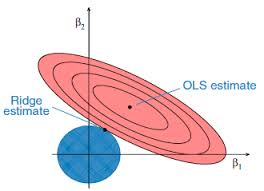
\includegraphics[height=2in]{ridge-constraint}
\footnote{onlinecourses.science.pse.edu}
\end{frame}
\begin{frame}
  \frametitle{Longley Data:  library(MASS); data(longley)}

\vspace{-12pt}

\begin{knitrout}
\definecolor{shadecolor}{rgb}{0.969, 0.969, 0.969}\color{fgcolor}

{\centering 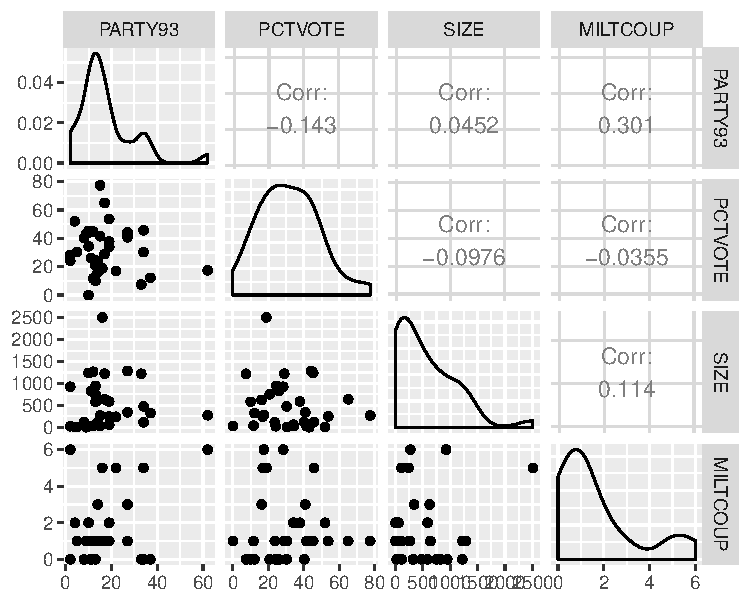
\includegraphics[width=\maxwidth]{figure/data-1} 

}



\end{knitrout}
\end{frame}

\begin{frame}[fragile]
  \frametitle{OLS}
\begin{small}
\begin{verbatim}
> longley.lm = lm(Employed ~ ., data=longley)
> summary(longley.lm)

Coefficients:
               Estimate Std. Error t value Pr(>|t|)
(Intercept)  -3.482e+03  8.904e+02  -3.911 0.003560 **
GNP.deflator  1.506e-02  8.492e-02   0.177 0.863141
GNP          -3.582e-02  3.349e-02  -1.070 0.312681
Unemployed   -2.020e-02  4.884e-03  -4.136 0.002535 **
Armed.Forces -1.033e-02  2.143e-03  -4.822 0.000944 ***
Population   -5.110e-02  2.261e-01  -0.226 0.826212
Year          1.829e+00  4.555e-01   4.016 0.003037 **
---
Signif. codes:  0 '***' 0.001 '**' 0.01 '*' 0.05 '.' 0.1 ' ' 1

Residual standard error: 0.3049 on 9 degrees of freedom
Multiple R-squared: 0.9955,	Adjusted R-squared: 0.9925
F-statistic: 330.3 on 6 and 9 DF,  p-value: 4.984e-10
\end{verbatim}
\end{small}
\end{frame}


\begin{frame}[fragile]  \frametitle{Ridge Regression}
\begin{knitrout}
\definecolor{shadecolor}{rgb}{0.969, 0.969, 0.969}\color{fgcolor}\begin{kframe}
\begin{alltt}
\hlcom{# from library MASS}
\hlstd{longley.ridge} \hlkwb{=} \hlkwd{lm.ridge}\hlstd{(Employed} \hlopt{~} \hlstd{.,} \hlkwc{data}\hlstd{=longley,}
                         \hlkwc{lambda}\hlstd{=}\hlkwd{seq}\hlstd{(}\hlnum{0}\hlstd{,} \hlnum{0.1}\hlstd{,} \hlnum{0.0001}\hlstd{))}
\hlcom{# lambda = k in notes}

\hlkwd{summary}\hlstd{(longley.ridge)}
\end{alltt}
\begin{verbatim}
##        Length Class  Mode   
## coef   6006   -none- numeric
## scales    6   -none- numeric
## Inter     1   -none- numeric
## lambda 1001   -none- numeric
## ym        1   -none- numeric
## xm        6   -none- numeric
## GCV    1001   -none- numeric
## kHKB      1   -none- numeric
## kLW       1   -none- numeric
\end{verbatim}
\end{kframe}
\end{knitrout}
\end{frame}


\begin{frame}[fragile]  \frametitle{Ridge Trace Plot}
\begin{knitrout}
\definecolor{shadecolor}{rgb}{0.969, 0.969, 0.969}\color{fgcolor}
\includegraphics[width=\maxwidth]{figure/ridgetrace-1} 

\end{knitrout}
\end{frame}


\begin{frame}[fragile]\frametitle{Choice of $k$}
\begin{knitrout}
\definecolor{shadecolor}{rgb}{0.969, 0.969, 0.969}\color{fgcolor}\begin{kframe}
\begin{alltt}
\hlstd{k} \hlkwb{=} \hlkwd{seq}\hlstd{(}\hlnum{0}\hlstd{,} \hlnum{0.1}\hlstd{,} \hlnum{0.0001}\hlstd{)}
\hlstd{n.k} \hlkwb{=} \hlkwd{length}\hlstd{(k); n} \hlkwb{=} \hlkwd{nrow}\hlstd{(longley)}
\hlstd{cv.lambda} \hlkwb{=} \hlkwd{matrix}\hlstd{(}\hlnum{NA}\hlstd{, n, n.k)}

\hlstd{rmse.ridge} \hlkwb{=} \hlkwa{function}\hlstd{(}\hlkwc{data}\hlstd{,} \hlkwc{i}\hlstd{,} \hlkwc{j}\hlstd{,} \hlkwc{k}\hlstd{) \{}
  \hlstd{m.ridge} \hlkwb{=} \hlkwd{lm.ridge}\hlstd{(Employed} \hlopt{~} \hlstd{.,} \hlkwc{data} \hlstd{= data,} \hlkwc{lambda}\hlstd{=k[j],}
                          \hlkwc{subset} \hlstd{=} \hlopt{-}\hlstd{i)}
  \hlstd{yhat} \hlkwb{=} \hlkwd{scale}\hlstd{(data[i,}\hlnum{1}\hlopt{:}\hlnum{6}\hlstd{,} \hlkwc{drop}\hlstd{=F],}\hlkwc{center} \hlstd{= m.ridge}\hlopt{$}\hlstd{xm,}
                       \hlkwc{scale} \hlstd{= m.ridge}\hlopt{$}\hlstd{scales)} \hlopt
                \hlstd{m.ridge}\hlopt{$}\hlstd{coef} \hlopt{+} \hlstd{m.ridge}\hlopt{$}\hlstd{ym}
\hlstd{(yhat} \hlopt{-} \hlstd{data}\hlopt{$}\hlstd{Employed[i])}\hlopt{^}\hlnum{2}
\hlstd{\}}

\hlkwa{for} \hlstd{(i}  \hlkwa{in} \hlnum{1}\hlopt{:}\hlstd{n)  \{}
  \hlkwa{for} \hlstd{(j} \hlkwa{in} \hlnum{1}\hlopt{:}\hlstd{n.k) \{}
    \hlstd{cv.lambda[i,j]} \hlkwb{=} \hlkwd{rmse.ridge}\hlstd{(longley, i, j, k)}
  \hlstd{\}}
\hlstd{\}}
\end{alltt}
\end{kframe}
\end{knitrout}
\end{frame}

\begin{frame}[fragile] \frametitle{Cross Validation Error}
\begin{knitrout}
\definecolor{shadecolor}{rgb}{0.969, 0.969, 0.969}\color{fgcolor}\begin{kframe}
\begin{alltt}
\hlstd{cv.error} \hlkwb{=} \hlkwd{apply}\hlstd{(cv.lambda,} \hlnum{2}\hlstd{, mean)}
\hlkwd{plot}\hlstd{(k, cv.error,} \hlkwc{type}\hlstd{=}\hlstr{"l"}\hlstd{)}
\end{alltt}
\end{kframe}
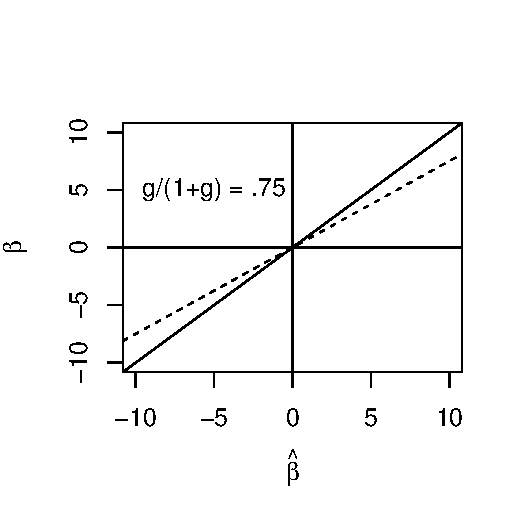
\includegraphics[width=\maxwidth]{figure/unnamed-chunk-1-1} 

\end{knitrout}
Best $k$ = 0.0028

\end{frame}

\begin{frame}[fragile]
\frametitle{Generalized Cross-validation}
\begin{small}
\begin{knitrout}
\definecolor{shadecolor}{rgb}{0.969, 0.969, 0.969}\color{fgcolor}\begin{kframe}
\begin{alltt}
\hlkwd{select}\hlstd{(}\hlkwd{lm.ridge}\hlstd{(Employed} \hlopt{~} \hlstd{.,} \hlkwc{data}\hlstd{=longley,}
         \hlkwc{lambda}\hlstd{=}\hlkwd{seq}\hlstd{(}\hlnum{0}\hlstd{,} \hlnum{0.1}\hlstd{,} \hlnum{0.0001}\hlstd{)))}
\end{alltt}
\begin{verbatim}
## modified HKB estimator is 0.004275357 
## modified L-W estimator is 0.03229531 
## smallest value of GCV  at 0.0028
\end{verbatim}
\begin{alltt}
\hlstd{best.k} \hlkwb{=} \hlstd{longley.ridge}\hlopt{$}\hlstd{lambda[}\hlkwd{which.min}\hlstd{(longley.ridge}\hlopt{$}\hlstd{GCV)]}
\hlstd{longley.RReg} \hlkwb{=} \hlkwd{lm.ridge}\hlstd{(Employed} \hlopt{~} \hlstd{.,} \hlkwc{data}\hlstd{=longley,}
                        \hlkwc{lambda}\hlstd{=best.k)}
\hlkwd{coef}\hlstd{(longley.RReg)}
\end{alltt}
\begin{verbatim}
##                GNP.deflator           GNP    Unemployed  Armed.Forces 
## -2.950348e+03 -5.381450e-04 -1.822639e-02 -1.761107e-02 -9.607256e-03 
##    Population          Year 
## -1.185103e-01  1.557856e+00
\end{verbatim}
\end{kframe}
\end{knitrout}

\end{small}

\end{frame}








\begin{frame}
  \frametitle{Priors on $k$}

$\X$ is centered and standardized
  \begin{eqnarray*}
  \Y  & =  &\one \beta_0 + \X  \b + \eps
  \end{eqnarray*}

Hierarchical prior \pause
\begin{itemize}
\item $p(\beta_0,  \phi \mid \b, \kappa) \propto \phi^{-1}$ \pause
\item $\b \mid \phi, \kappa \sim \N(\zero, \I (\phi \kappa )^{-1})$ \pause
\item prior on $\kappa$?  \pause

\item Take $$\kappa \mid \phi \sim  \Gam(1/2, 1/2)$$ \pause

\item What is induced prior on $\b \mid \phi$?
\end{itemize}
\end{frame}


\begin{frame}
  \frametitle{Posterior Distributions}
Joint Distribution
  \begin{itemize}
 \item $\beta_0, \b, \phi \mid \kappa, \Y$  Normal-Gamma family given $\Y$
   and $\kappa$ \pause
  \item $\kappa \mid \Y$  not tractable \pause
  \end{itemize}
Obtain marginal for  $\b$ via  MCMC \pause
%\begin{itemize}

Pick initial values $\beta_0^{(0)}, \b^{(0)},
  \phi^{(0)}$, \pause \\

Set  $t = 1$

\begin{enumerate}
 \item Sample $\kappa^{(t)} \sim p(\kappa \mid \beta_0^{(t-1)},
    \b^{(t-1)}, \phi^{(t-1)}, \Y)$ \pause
\item Sample $\beta_0^{(t)}, \b^{(t)}, \phi^{(t)} \mid \kappa(t),
     \Y$ \pause
\item  Set $t = t + 1$ and repeat until $t > T$ \pause
\end{enumerate}
Use Samples  $\beta_0^{(t)}, \b^{(t)}, \phi^{(t)}, \kappa^{(t)}$ for $t
= B, \ldots, T$ for inference

\end{frame}

\begin{frame} \frametitle{JAGS}
JAGS = Just Another Gibbs Sampler \pause

\begin{itemize}
\item scripting language to express sampling models and priors \pause
\item "derives" full conditional distributions \pause
\item integrates with R \pause
\item typically faster than interpreted R code \pause
\item accounts for uncertainty about $k$ \pause
\end{itemize}

How would you compare Bayes predictions with Ridge with Cross-validation?
\end{frame}
\end{document}

